\chapter{Introduction}

A spectral image contains rich information in spectral domain by capturing the
electromagnetic (EM) reflectance at a number of wavelengt in each pixel.
An ordinary color camera, for example, captures the EM reflectance at three
broad spectral bands roughly at the wavelength corresponding to red
($0.6\,\mu$m-$0.68\,\mu$m), green ($0.53\,\mu$m-$0.57\,\mu$m) and blue
($0.42\,\mu$m-$0.48\,\mu$m) in the visible range.
A spectral camera, rather than only receiving signals at few spectral bands,
captures over a hundred spectral bands spanning the visible range and the
infrared region.

In remote sensing and Earth science applications, a popular hyperspectral
sensor named "Airborne Visible/InfraRed Imaging Spectrometer" (AVIRIS)
captures hyperspectral images (HSIs) at $224$ spectral bands covering
wavelengths between $0.4\,\mu$m and $2.5\,\mu$m at norminally $10\,$nm
intervals.
Usually the AVIRIS sensor is placed at $20\,$km altitude inspecting the Earth
surface at about $20\,$m ground sampling distance (GSD), which is defined as
the actual ground distance between neighbouring pixels in the HSI
\cite{COMP_AVIRIS_HYPERION_FOR_HSI_MINERAL_MAPPING,
      IMG_SPECTROSCOPY_AND_AVIRIS,
      EXPL_RELATION_BTW_INFO_AND_SNR_AND_SPATIAL_RESOL_IN_AVIRIS}.
Suppose the spatial dimension of HSIs taken by a AVIRIS sensor has $m \times n$
pixels and the spectral dimension contains $\lambda$ bands.
The resultant HSI is an image cube with $m \times n \times \lambda$ values, as
illustrated in Figure \ref{fig:INTRO_HSI}.

\begin{figure}[t]
    \centering
    \resizebox{0.98\linewidth}{!}{
        \begin{tikzpicture}
            \node at (0,0) [xshift=  -4cm,yshift=   0cm](nHSI){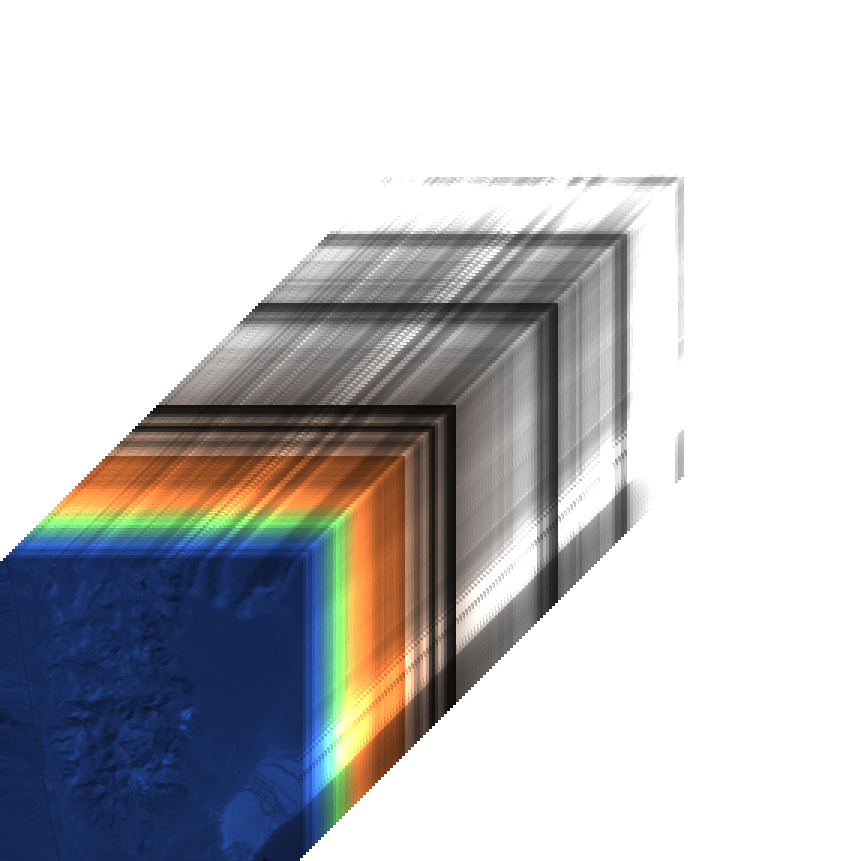
\includegraphics[width=8cm]{./fig/fig_01Intro/2D_HSI_Gen_copy/HSI}};
            \node at (nHSI)[xshift=  -5cm,yshift=-2.6cm](nm)  {\large $m$};
            \node at (nm)  [xshift= 0.7cm,yshift= 1.5cm](nmAr1) {$\;$} ;
            \node at (nm)  [xshift= 0.7cm,yshift=-1.5cm](nmAr2) {$\;$} ;
            \draw[<->] (nmAr1.-90) -- (nmAr2.90) ;
            \node at (nHSI)[xshift=-2.6cm,yshift=-4.5cm](nn)  {\large $n$} ;
            \node at (nn)  [xshift=-1.6cm,yshift= 0.2cm](nnAr1) {$\;$} ;
            \node at (nn)  [xshift= 1.6cm,yshift= 0.2cm](nnAr2) {$\;$} ;
            \draw[<->] (nnAr1.0) -- (nnAr2.180) ;
            \node at (nHSI)[xshift=-2.8cm,yshift= 1.0cm](nl)  {\large $\lambda$} ;
            \node at (nl)  [xshift=-1.5cm,yshift=-2.0cm](nlAr1) {$\;$} ;
            \node at (nl)  [xshift= 2.0cm,yshift= 1.5cm](nlAr2) {$\;$} ;
            \draw[<->] (nlAr1.45) -- (nlAr2.-135) ;
            \node at (0,0) [xshift=   1cm,yshift= 1.0cm](nRGB){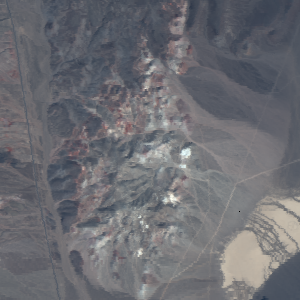
\includegraphics[width=2.5cm]{./fig/fig_01Intro/2D_HSI_Gen_copy/RGB}} ;
            \node at (nRGB)[xshift= 1.5cm,yshift=-3.0cm](nR)  {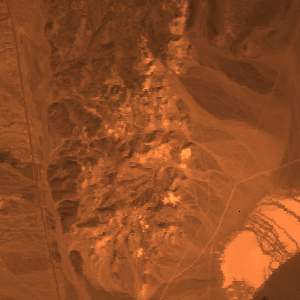
\includegraphics[width=2.5cm]{./fig/fig_01Intro/2D_HSI_Gen_copy/R}} ;
            \node at (nRGB)[xshift= 0.0cm,yshift=-3.5cm](nG)  {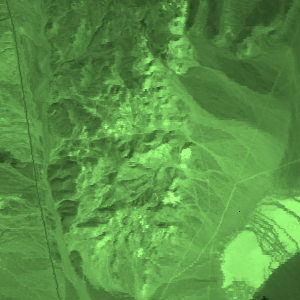
\includegraphics[width=2.5cm]{./fig/fig_01Intro/2D_HSI_Gen_copy/G}} ;
            \node at (nRGB)[xshift=-1.5cm,yshift=-4.0cm](nB)  {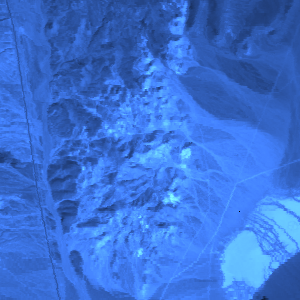
\includegraphics[width=2.5cm]{./fig/fig_01Intro/2D_HSI_Gen_copy/B}} ;
            \node at (nHSI)[xshift= 0.7cm,yshift=-3.5cm](nArr){$\;$} ;
            \node at (nArr)[xshift=-1.2cm,yshift=   0cm](nBAr1){$\;$} ;
            \node at (nArr)[xshift= 0.2cm,yshift=   0cm](nBAr2){$\;$} ;
            \node at (nArr)[xshift=-0.7cm,yshift= 0.2cm](nGAr1){$\;$} ;
            \node at (nArr)[xshift= 0.7cm,yshift= 0.2cm](nGAr2){$\;$} ;
            \node at (nArr)[xshift=-0.2cm,yshift= 0.4cm](nRAr1){$\;$} ;
            \node at (nArr)[xshift= 1.2cm,yshift= 0.4cm](nRAr2){$\;$} ;
            \draw          [blue ,->] (nBAr1.0) -- (nBAr2.180) ;
            \draw          [green,->] (nGAr1.0) -- (nGAr2.180) ;
            \draw          [red  ,->] (nRAr1.0) -- (nRAr2.180) ;
            \draw          [decorate,
                            decoration={brace,amplitude=10pt},
                            xshift=   1cm,yshift=-0.7cm]
                            (-2.7,0.0) -- (2.7,0.0) ;
        \end{tikzpicture}
    }
    \caption{HSI over an Earth surface and its conversion to ordinary color image.}
    \label{fig:INTRO_HSI}
\end{figure}

Hyperspectral unmixing and classification belong to a class of quantitative
analysis techniques that retrieve useful information from the pixels of HSIs.
These analysis have great potential in applications where the image scenes
tend to be large and complex, such as remote sensing, Earth science,
industrial resource exploration, aircraft-based systems, agricultural science
and wide area monitoring, or in small scale laboratory-based studies like food
quality analysis, chemical spectroscopy, biomedical science and forensic
science
\cite{IMG_SPECTROMETRY_FOR_EARTH_REMOTE_SENSING,
      ADV_IN_HS_REMOTE_SENSING_FOR_GEO_MAP,
      A_REVIEW_ON_APPL_OF_NIR_SPECTRO_AND_CHEM_FOR_AGROFOOD_PROC_INDST,
      HSI_FOR_FOOD_APPL,
      APPL_OF_ICA_WITH_JADE_ALGO_AND_NIR_HSI_FOR_REVEALING_FOOD_ADULTERATION},
to mention a few.
Usually an enhancement in the quality of an HSI in terms of spatial and
spectral resolution is beneficial to all hyperspectral imagery applications.
% identification, classification, mapping and unmixing.
In this thesis, the enhancement of HSIs in spatial and spectral quailty,
called hyperspectral super-resolution (HSR), for remote sensing purpose is
discussed.

\section{Overview of the Hyperspectral Super-resolution (HSR)}
\label{sec:HSR}
In geoscience and Earth science research, a number of industries have launched
satellites for Earth observation missions.
These projects include Sentinel, Landsat, RapidEye, QuickBird, EnMAP, AVIRIS,
HYPXIM, CHRIS, HISUI, Hyperion, DESIS, PRISMA, SHALOM, etc.
The resolution characteristics of the aforementioned wide spectrum of remote
sensing instruments are summarized in Figure \ref{fig:INTRO_HSMSSensors_Res}
\cite{HSMS_DATA_FUSION_A_COMPARATIVE_REVIEW}
in which more desirable sensors characteristics are marked in the purple
region; the hyperspectral (HS) and multispectral (MS) sensors are marked by
the blue dots and red dots, respectively.
From the figure we see that an ideal hyperspectral sensor should have small
GSD and large amount of spectral bands within a desired wavelength range.
However, in practice, hyperspectral sensors with such high spatial and
spectral resolution are not common due to hardward limitation, \ie we are
inevitably required to have a trade-off between the two resolutions.
\begin{figure}[t]
    \centering
    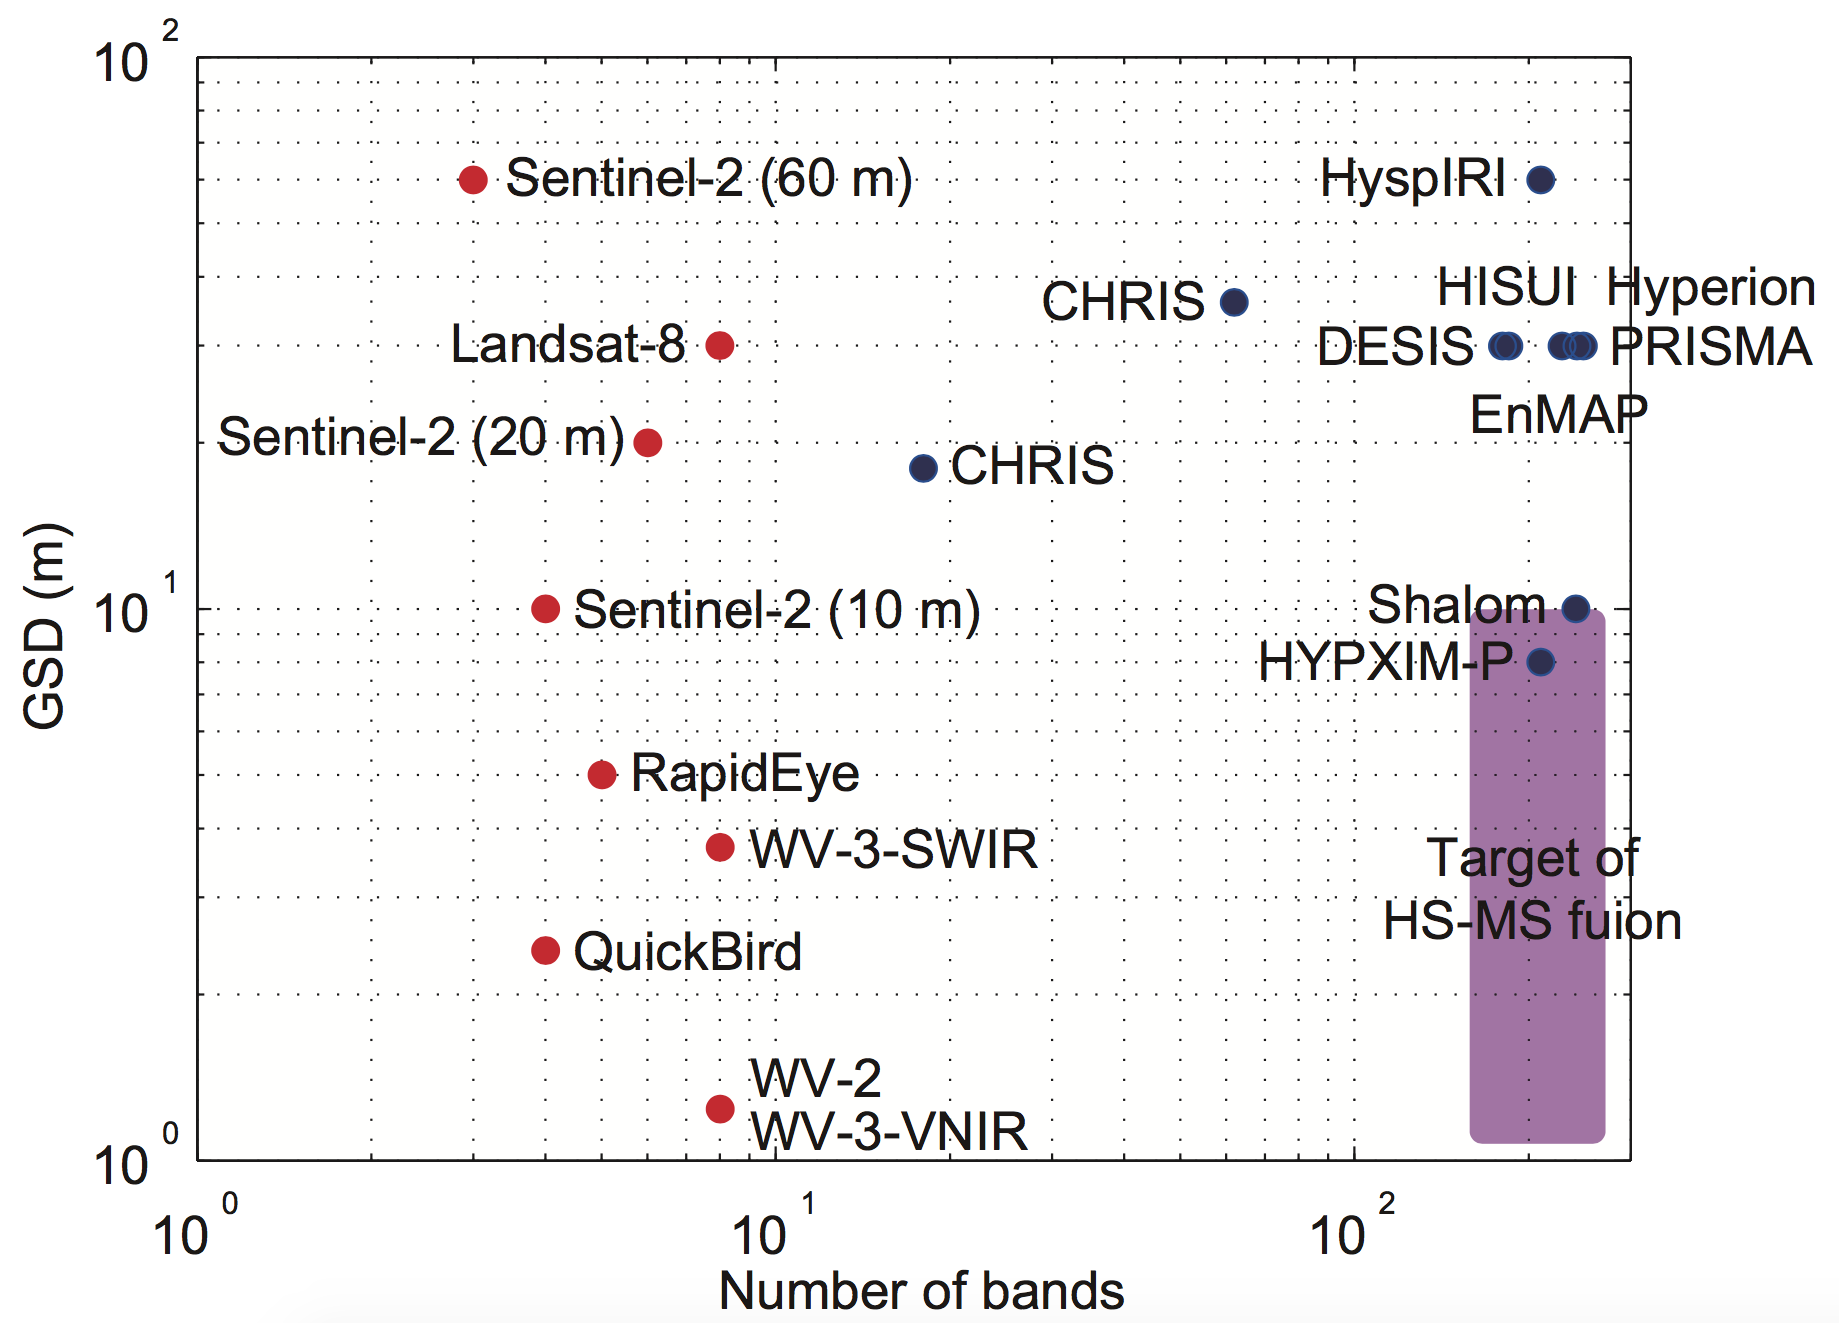
\includegraphics[width=.75\textwidth]{./fig/fig_01Intro/Introduction_HSMSSensors_Res}
    \caption{Resolutions of the latest remote satellite sensors
             \cite{HSMS_DATA_FUSION_A_COMPARATIVE_REVIEW}.}
    \label{fig:INTRO_HSMSSensors_Res}
\end{figure}

In this thesis, for ease of presentation, we define images with high
spectral resolution and low spatial resolution as hyperspectral (HS) images;
images with low spectral resolution and high spatial resolution as
multispectral (MS) images; images with high resolution in both spatial and
spectral domain as super-resolution (SR) images.
HSR estimates the SR image of a scene from its HS and MS observations such
that the combined image at most possesses the spectral resolution of the
former and spatial resolution of the latter (Figure \ref{fig:fusion_flow}).
\begin{figure}[t]
    \centering
    \resizebox{0.98\linewidth}{!}{
        \begin{tikzpicture}
            [dot/.style={circle,draw=black,fill=white,inner sep=5pt,minimum size=5pt}]
            \node at (0,0) [dot,draw=black,very thick ](n+)  {\Huge +};
            \node at (n+)  [xshift= -5cm,yshift=   3cm](nHS) {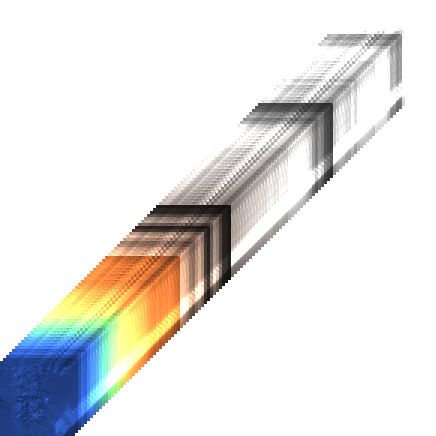
\includegraphics[width=5cm]{./fig/fig_01Intro/2D_HSI_Gen_copy/HS} };
            \node at (n+)  [xshift= -5cm,yshift=  -3cm](nMS) {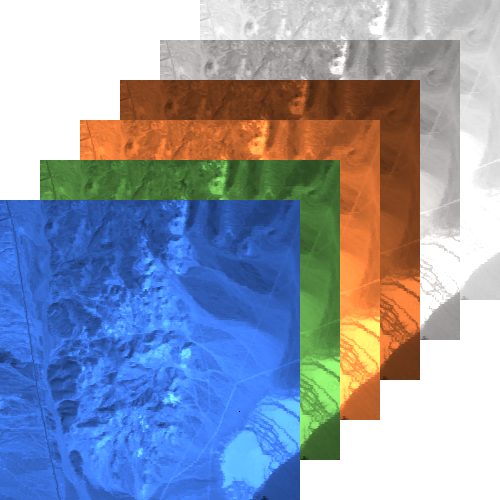
\includegraphics[width=5cm]{./fig/fig_01Intro/2D_HSI_Gen_copy/MS} };
            \node at (n+)  [xshift=  7cm,yshift=   0cm](nHSI){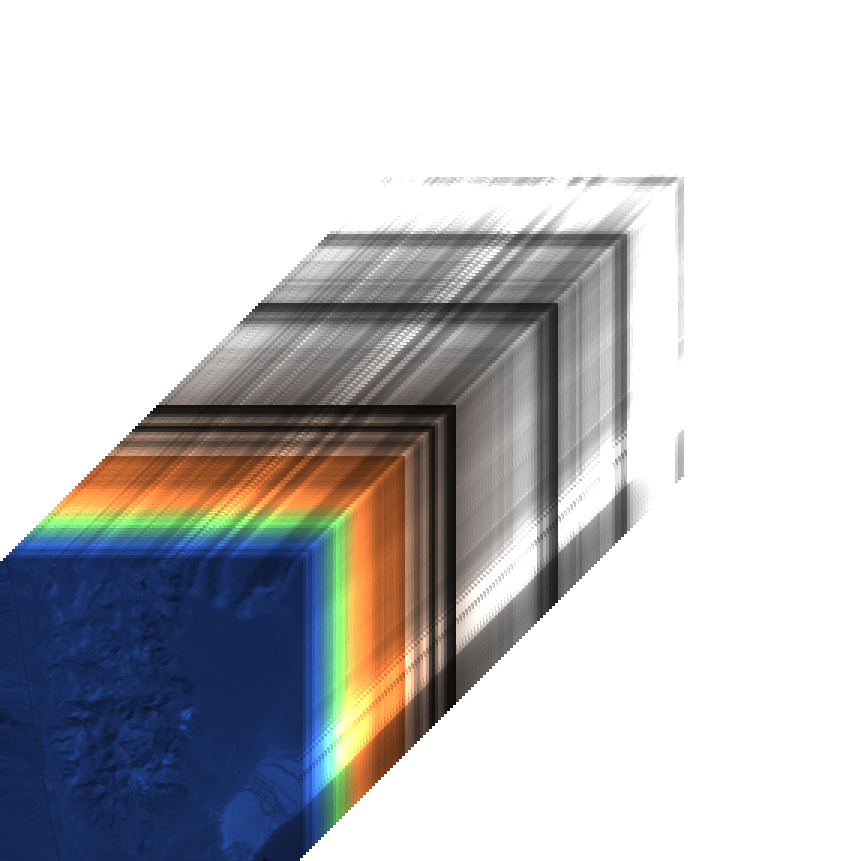
\includegraphics[width=8cm]{./fig/fig_01Intro/2D_HSI_Gen_copy/HSI}};
            \node at (n+)  [xshift=1.4cm,yshift= 1.2cm]      {\Large HSR                             };
            \node at (nHS) [xshift=  1cm,yshift=-1.5cm]      {\Large HS Image                        };
            \node at (nMS) [xshift=  1cm,yshift= 3.2cm]      {\Large MS Image                        };
            \node at (nHSI)[xshift=  1cm,yshift= 3.0cm]      {\Large SR Image                        };
            \draw[-{>[scale=2.5,length=5,width=6]},line width=1.2] (nHS.-30) -- (n+.140);
            \draw[-{>[scale=2.5,length=5,width=6]},line width=1.2] (nMS.30)  -- (n+.220);
            \draw[-{>[scale=2.5,length=5,width=6]},line width=1.2] (n+.0)  -- (nHSI.180);
        \end{tikzpicture}
    }
    \caption{Hyperspectral super-resolution from low resolution HS and MS images.}
    \label{fig:fusion_flow}
\end{figure}
Many approaches have been studied including Component Substitution (CS)
\cite{HSMSEXISTAPPROACH_CS_IHS,
      HSMSEXISTAPPROACH_CS_ENHANCING_MS_BY_PAN,
      HSMSEXISTAPPROACH_CS_IMPROVE_CS},
Multiresolution Analysis (MRA)
\cite{HSMSEXISTAPPROACH_MRA_SMOOTH_FILTER_IMG_FUSION,
      HSMSEXISTAPPROACH_MRA_MTF},
Bayesian approach
\cite{HSMSEXISTAPPROACH_BAYESIAN_STOC_MIX_MODEL_HSR,
      HSMSEXISTAPPROACH_BAYESIAN_MAP_ESTIMATE_HSR,
      HSMSEXISTAPPROACH_BAYESIAN_HSR_BY_MS}
and spectral unmixing
\cite{CNMF,
      HSMSEXISTAPPROACH_MF_NMFPAN,
      HSR_MF,
      HSMSEXISTAPPROACH_MF_SPAT_SPEC_IMG_FUSION,
      HSMSEXISTAPPROACH_MF_HSR_LOCAL_LOWRANK,
      HSMSEXISTAPPROACH_MF_JOINT_HSR_UNMIX_INTERACT_FEEDBACK}.
The competitiveness of these classes of methods have been summarized and
reviewed in
\cite{HS_PANSHARPENING_A_REVIEW,HSMS_DATA_FUSION_A_COMPARATIVE_REVIEW}.
In this thesis, we focus on HSR by spectral unmixing.

\section{Overview of Convex Optimization}
Some basic concepts of convex optimization are reviewed in this section.
First of all, a few definitions on convex sets and convex functions are
given before further discussion on convex optimization problems.

\subsection{Convex Sets}
A set $\mathcal S \subseteq \R^N$ is convex if the line segment drawn from any
two points in $\mathcal S$ lies in $\mathcal S$, \ie
$\forall \; \bm x,\bm y \in \mathcal S$,
\begin{equation}
    \alpha \bm x + (1-\alpha) \bm y \in \mathcal S, \;\;\;
    \forall \; \alpha\in[0,1].
\end{equation}
Some examples of convex sets are given as
\begin{itemize}
    \item $\R^n_+$ (nonnegative orthant);
    \item $\{\bm x \in \R^2_+ \;|\; x_1 - 3x_2 \leq 0, -2x_1 + 3x_2 \leq 0\}$
          (a convex cone);
    \item $\{\bm x \in \R^n \;|\; \Vert \bm x \Vert_2 \leq 1\}$ (unit $\ell_2$-norm ball);
    \item $\{\bm x \in \R^n \;|\; \Vert \bm x \Vert_1 \leq 1\}$ (unit $\ell_1$-norm ball);
    \item $\{\bm x \in \R^n \;|\; \vert x_i \vert \leq 1\}$ (a box).
\end{itemize}

\subsection{Convex Functions}
A function $f:\mathcal S\rightarrow\R$ is said to be convex if $\mathcal S$ is
a convex set and $f$ satisfies
\begin{equation}
    f(\alpha \bm x + (1-\alpha) \bm y) \leq
    \alpha f(\bm x) + (1-\alpha) f(\bm y), \;\;\;
    \forall \; \bm x \; , \; \bm y \in \R^N \; , \; \alpha \in [0,1].
    \label{eq:convex_function_definition_1}
\end{equation}
If $f(\bm x)$ is differentiable in $\bm x$ within $\mathcal S$, then the
condition in \eqref{eq:convex_function_definition_1} is equivalent to
\begin{equation}
    f(\bm y) \geq f(\bm x) + \nabla f(\bm x)\Tr (\bm y - \bm x),
    \label{eq:first_order_condition}
\end{equation}
where $\nabla f(\bm x)$ denotes the gradient of $f$ at point $\bm x$.
\eqref{eq:first_order_condition} is called the first order condition in the
literature.

\subsection{Convex Optimization Problems}
Consider the following optimization problem.
\begin{equation}
    \begin{array}{cl}
        \underset{\bm x}{\min} & f(\bm x) \\
        \text{s.t.}            & \bm x \in \mathcal S,
    \end{array}
    \label{eq:general_convex_optimization_problem}
\end{equation}
where $\bm x$ is the decision variable, $f$ is the objective function in
$\bm x$ and $\mathcal S$ is the feasible set of $\bm x$.
If function $f$ and feasible set $\mathcal S$ of
\eqref{eq:general_convex_optimization_problem} are both convex, then
\eqref{eq:general_convex_optimization_problem} is called a convex optimization
problem.
A convex optimization problem has the following properties:
\begin{itemize}
    \item [1)] Any locally optimal points are globally optimal;
    \item [2)] If $f$ is differentiable everywhere in $\mathcal S$, then the
               first-order condition holds;
    \item [3)] If $\bm x^* \in \mathcal S$ is a minimizer of problem
               \eqref{eq:general_convex_optimization_problem}, then
               \begin{equation}
                   \nabla f(\bm x^*)\Tr (\bm y - \bm x^*) \geq 0
                   \;\;\; \forall \; \bm y \in \mathcal S.
               \end{equation}
\end{itemize}

\section{Significance of Convex Optimization}
%Convex optimization problems can be solved easily and efficiently.
If a real world problem can be formulated as a convex optimization problem,
then in general this problem can be solved exactly, efficiently and easily by
methods like first order gradient method (FOGM), interior point method and
many more.
History has shown that convex optimization has been benefitting many practical
situations including automatic control
systems, signal estimation and detection, communications, network design and
data modelling while there are abundant reliable computer software that help
solve their problems.


\section{Coordinate Descent Algorithms}
A coordinate descent algorithm solves optimization problems by successively
performing approximate minimization along coordinate directions (or coordinate
hyperplanes)
\cite{COORD_DESCENT_ALGO}.
It is an iterative method in which each iterate is obtained by fixing most
components of the decision variable vector $\bm x$ at their values from the
current iteration, and approximately minimizing the objective with respect to
the remaining components.
Typically, this approach lowers the dimensions of the subproblems and thus
motivates people solving the subproblems and updating the variables in an
easier and more efficient way compared with handling the full problem and the
full variable vector.

Specifically, consider the decision variable $\bm x \in \mathcal X$ that is
decomposable into $N$ blocks as $\bm x \coloneqq (\bm x_1,\cdots,\bm x_N)$;
$\mathcal X \coloneqq \mathcal X_1 \times \cdots \mathcal X_N$ as the feasible
set; $f:\mathcal X \rightarrow \R$ as the objective function that can be
expressed as $f(\bm x_1,\cdots,\bm x_N)$; the function that depends on
$\bm x_i$ as $f_i(\bm x_1,\cdots,\bm x_i,\cdots,\bm x_N)$.
A general optimization problem of the form
\begin{equation}
    \begin{array}{cl}
        \underset{\bm x}{\min} & f(\bm x) \\
        \text{s.t.}            & \bm x \in \mathcal X
    \end{array}
\end{equation}
can be solved to a stationary point by a coordinate descent algorithm
described below.
\begin{algorithm}
    \caption{Coordinate Descent Algorithm}
    \label{alg:CD}
    \begin{algorithmic}[1]
        \Require{$\bm x\iter{0} \in \mathcal{X}$.}
        \For{$k=1,2,\cdots$ until stopping criteria holds}
            \State{$\bm x\iter{k,0} \gets \bm x\iter{k}$.}
            \For{$i=1,\cdots,N$}
                \State{Update:
                       \begin{equation}
                           \bm x_i\iter{k,i}
                           \gets
                           \begin{cases}
                               \underset{\bm x_j \in \mathcal X_i}{\min}
                               f_i(\bm x_1    \iter{k,i  },\cdots,
                                   \bm x_{j-1}\iter{k,i  },
                                   \bm x_j                ,
                                   \bm x_{j+1}\iter{k,i-1},\cdots,
                                   \bm x_N    \iter{k,i-1})
                               & j = i, \\
                               x_j\iter{k,i-1}
                               & j\neq i.
                           \end{cases}
                       \end{equation}
                      }
            \EndFor
            \State{$\bm x\iter{k+1} \gets \bm x\iter{k,i}$.}
        \EndFor
        \Ensure{$\bm x\iter{k+1}$.}
    \end{algorithmic}
\end{algorithm}

At the $k\thtxt$ iteration, the above CD algorithm separates the full problem
$\underset{\bm x\in\mathcal X}{\min}\;f(\bm x)$ into $N$ subproblems which
approximate $f$ along each coordinate direction at the current state
$x\iter{k}$.
The algorithm then exactly solves each subproblem in a cyclic sense.
Note that the variable update is not necessarily ordered in a cyclic manner.
It could be a randomized sequence between $1$ and $N$ or an order following
the coordinate index whose gradient component has the maximal absolute value,
as illustrated in
\cite{NESTEROV_BCD_HUGE_PROBLEM}.

CD algorithm can be easily extended to a Block-CD (BCD) algorithm by each time
considering the decision variable vector $\bm x$ along multiple coordinate
directions (or coordinate hyperplanes).
Examples of BCD benefitting a wide range of applications can be found in
\cite{BCD_APPL_STAT_TOMOGRAPHY,
      BCD_APPL_DIFF_TOMOGRAPHY,
      BCD_APPL_BCD_FOR_MULTITASK_LASSO_NEURAL_DISCOV,
      BCD_APPL_PROTEIN_LOOP,
      BCD_APPL_OD_MATRIX_ADJ_PROBL,
      BCD_APPL_BIOFEATURE,
      BCD_APPL_SPARSE_COV_EST,
      BCD_APPL_LARGESCALE_LINEAR_SVM}.

\section{Contributions}
In this thesis we investigate the efficiency and effectiveness of BCD using
FOGMs to tackle the HSR problem.
Specifically, the non-convex HSR problem is separable into two block convex
subproblems that can be individually solved by FOGMs.
We study the effect of exactness of solving the subproblems towards the full
HSR performance in terms of accuracy and runtime.
We find that with inexact solving of the subproblems (\ie inexact BCD), the
HSR can still be solved to a stationary point while the accuracy can be
preserved and, more importantly, the runtime is largely reduced compared to
state-of-the-art algorithms.
%The importance of the 
%The study goes through two state-of-the-art problem formulations.
%The contributions is that a fast framework of FOGMs is proposed with the
%benefit being that the computation time required is much less than that
%required by the state of the arts while a comparable HSR quality is achieved.

\section{Organization}
The organization of this thesis is as follows.
Chapter 2 describes the system model and the HSR problem.
Chapter 3 describes how FOGMs may solve a quadratic program in detail.
After that the HSR problem is shown to be a two block quadratic program that
can be handled by BCD algorithms.
Chapter 4 presents synthetic and semi-real simulations to compare the
performance by BCD algorithms using FOGMs and that by state-of-the-art
algorithms.
Chapter 5 summarizes this thesis.

